% Created 2016-08-17 Wed 14:38
\documentclass[tikz]{standalone}

\usepackage[utf8]{inputenc}
\usepackage[T1]{fontenc}
\usepackage{helvet}
\usepackage{../../templates/msc}

\renewcommand{\familydefault}{\sfdefault}

\tikzset{
every picture/.style={
line width=1pt
}}

\usepackage{tikz}
\author{Holger Karl}
\date{\today}
\title{}

\usetikzlibrary{positioning,fit,calc}

\begin{document}
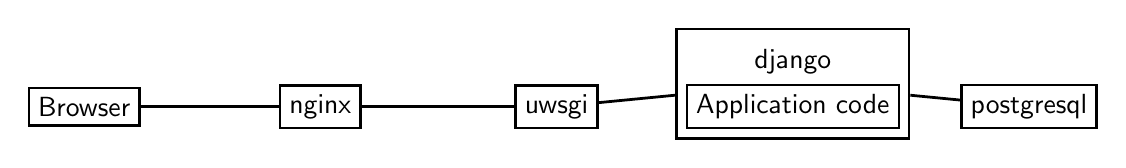
\begin{tikzpicture}[auto, xscale=3,
block/.style = {rectangle, draw=black, thick, align=left}]
\node[block] at (0,0) (b) {Browser}; 
\node[block] at (1,0)  (n)  {nginx}; 
\node[block] at (2,0)  (u) {uwsgi}; 
\node[block] at (3,0) (ac) {Application code};
\node[] (d)  [above=of ac.north, yshift=-1cm] {django }; 
\node[draw=black, fit=(ac) (d)]  (d) {}; 
\node[block] at (4,0)  (p) {postgresql}; 

\draw[-] (b) --(n); 
\draw[-] (n) --(u); 
\draw[-] (u) --(d); 
\draw[-] (d) --(p); 
  % \node [block]  at (0,1) (sender) {\textbf{Sender:} \\x = native data;\\px = pack(x);
  %   \\send(px);};
  % \node [block] at (2,3) (idl) {Data definition file};
  % \node [block] at (2,2) (idlcomp) {IDL compiler};
  % \node [block] at (1,1) (pack) {pack()}; 
  % \node [block] at (3,1) (unpack) {unpack()}; 
  % \node [block]  at (4,1) (receiver) {\textbf{Receiver:} \\px =  receive();\\x = unpack(px);
  %   \\//use native data in x };
  % %
  % \draw [->] (idl) -- (idlcomp); 
  % \draw [->] (idlcomp) -- (pack); 
  % \draw [->] (idlcomp) -- (unpack); 
  % \draw (-1,-1) -- (5,-1);
  % \draw [->] (sender) -- (0, -1); 
  % \draw [->] (4, -1) -- (receiver); 
  % \draw  [->] (sender.east) to [bend left=80] (pack.west) ; 
  % \draw  [->] (pack.west) to [bend left=45] (sender.east) ; 
  % \draw  [->] (receiver.west) to [bend left=45] (unpack.east) ; 
  % \draw  [->] (unpack.east) to [bend left=45] (receiver.west) ; 
  % \path (sender) edge [bend north ] node [right] {} (pack);
\end{tikzpicture}
\end{document}